\documentclass[10pt]{article}
\usepackage[polish]{babel}
\usepackage[utf8]{inputenc}
\usepackage[T1]{fontenc}
\usepackage{amsmath}
\usepackage{amsfonts}
\usepackage{amssymb}
\usepackage[version=4]{mhchem}
\usepackage{stmaryrd}
\usepackage{graphicx}
\usepackage[export]{adjustbox}
\graphicspath{ {./images/} }

\title{Zadania - etap II }

\author{}
\date{}


\begin{document}
\maketitle
\section*{(klasy 5 i 6 szkoły podstawowej)}
Zadanie 1. Dla liczb: \(x=\frac{4646}{6969}, y=\frac{5858}{8787}, a=\frac{24}{77}, b=\frac{2424}{7777}, c=\frac{242424}{777777}\), oblicz wartość wyrażenia \(w=\frac{(x+y) a}{b+c}\).

Zadanie 2. Obwód trójkąta równoramiennego jest równy 56 cm . Środek jednego z ramion połączono z wierzchołkiem przeciwległego kąta. Powstały w ten sposób dwa nowe trójkąty, z których jeden (zawierający podstawę trójkąta) ma obwód o 10 cm krótszy niż drugi trójkąt. Oblicz długości boków trójkąta równoramiennego.

Zadanie 3. Prostokąt \(A B C D\) podzielono na cztery prostokąty, jak na rysunku poniżej. Obwód prostokąta I jest równy 20, a obwód prostokąta II jest równy 30. Oblicz obwód prostokąta ABCD.\\
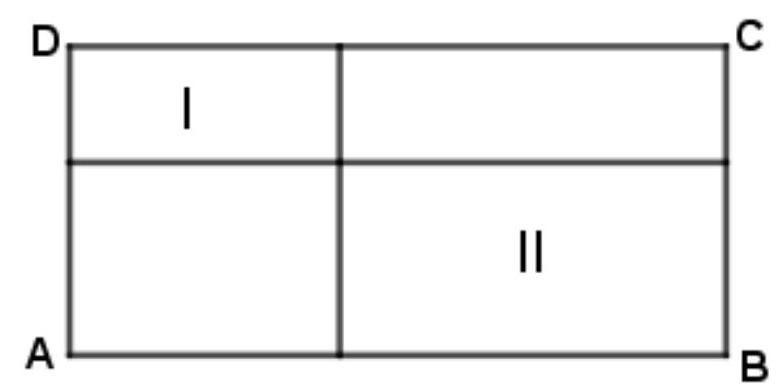
\includegraphics[max width=\textwidth, center]{2024_11_21_a91ed06327e40136c6d4g-1}

Zadanie 4. Oblicz: \(2010 \frac{7}{101} \cdot 2011 \frac{7}{101}-2009 \frac{7}{101} \cdot 2012 \frac{7}{101}\).

Zadanie 5. Między cyfry licznika i mianownika ułamka \(\frac{34}{61}\) wstaw po dwie takie same cyfry napisane w tej samej kolejności tak, aby otrzymany ułamek \(\frac{3 x y 4}{6 x y 1}\) był równy ułamkowi \(\frac{34}{61}\).


\end{document}